\section{A Particle in a Finite Square Well}
%By Matt Trawick

\makelabheader %(Space for student name, etc., defined in master.tex)

\bigskip

\begin{wrapfigure}[16]{r}{0.40\textwidth}
\begin{center}
\vspace{-0.1in}
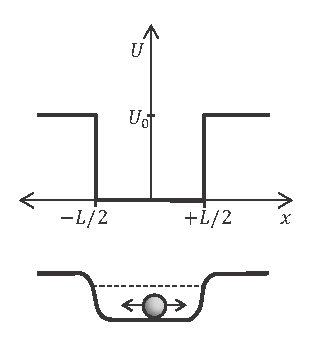
\includegraphics[width=0.34\textwidth]{particle_in_finite_well/finite_potential.eps}
\end{center}
\end{wrapfigure}

\textbf{Introduction}

Previously we looked at the case of a particle that was stuck inside a one-dimensional ``box''. 
Outside of this box, the potential energy $U(x)$ was infinite. This meant that the electron (or whatever) absolutely positively could not get out of the box, no matter how big its energy was. 
We called the box an ``infinite square well'' since the potential energy went to $U=\infty$ at the edges and beyond.

Now we'll play with potential wells that are finite, in the sense that the potential energy outside the edges does not go to infinity. The graph to the right shows an example.

It's hard to imagine a physical situation that has exactly the potential energy function shown, so think of the graph as a kind of limiting case of the situation shown in the lower picture: a bowling ball rolling back and forth in a valley with fairly strongly sloped hills around it.  You have to round the edges slightly to let the ball roll partway up the hills.  If the bowling ball has a total energy $E<U_0$ shown by the dashed line, then our classical intuition (and conservation of energy) would tell us that it can never escape from the well.  We say the ball is ``bound'' inside the well.

\bigskip

\textbf{Activity 1: Wave Functions and Bound States}

So let's see what the Schr\"odinger equation tells us about the wave function $\psi(x)$ for a particle inside a one-dimensional finite square well. The Schr\"odinger equation says that
$$-\frac{\hbar^2}{2m} \frac{d^2\psi(x)}{dx^2} + U(x)\psi(x) = E\psi(x),$$
where $U(x) = 0$ inside the well, and $U(x) = U_0$ outside the well. Inside the well, we already know
the answer from the previous lab: the $U(x)$ term drops out, and the possible solutions to $\psi(x)$ are
$$\psi(x)=A\sin(kx)$$
$$\psi(x)=A\cos(kx)$$
where $k=\sqrt{2mE/\hbar^2}$.

\begin{enumerate}[wide]
\item Now, let's look at $\psi(x)$ outside the box, say for $x > L/2$.  Here, we have to keep $U(x)$ in the Schr\"odinger equation:
$$\frac{d^2\psi(x)}{dx^2} = \frac{2m(U_0 - E)}{\hbar^2}\psi(x),$$
But now the constant $U_0 - E$ is \textit{positive}, so we are looking for a function $\psi(x)$ where if you take the second derivative of it, you get a \textit{positive} constant $2m(U_0 - E) / \hbar^2$ times that same function. What are two possible functions $\psi(x)$ that fit the bill?  (They differ only by a strategically placed negative sign.) 
\answerspace{0.5in}

\item Of the two equations you have written above for $\psi(x)$, one works great for $x < -L/2$, one works for $x > L/2$. Which is which?
\answerspace{0.5in}

\pagebreak[2]

In the region between the walls, the function will have to be made out of sines and cosines, and it will have to be continuous with the function outside the walls, as we'll discuss.  It is this center region and the continuity condition that will set up energy quantization, so that the wavefunction will depend on some integer-valued $n$.

To give yourself some sense of what $\psi(x)$ looks like for different values of energy $E$, open the following page in Internet Explorer:
$$\verb!http://webphysics.davidson.edu/physletprob/ch10_modern/default.html!$$
Click on \button{Finite Well} on the left hand side. This simulation shows a 1-dimensional box running from $x =-0.50$ to $x = +0.50$. The potential energy is shown as a red line at $U = 0$, with the ``infinite'' vertical walls just off screen. Initially, your particle has been given an energy of $E = 8.712$ (in some units), which leads to the ``ground state'' (n=1) function $\psi(x)$ shown in blue.

\item Draw sketches of $\psi(x)$ below for $E = 34$ and $E = 35$ (Type the numbers in the \button{Energy} box and hit \button{Enter}). Are either one of these a good-looking wave function for $\psi(x)$? Why or why not?
\answerspace{1.5in}

\item Now try some values between $E = 34$ and $E = 35$. What's the best value for this second lowest energy state? Check your answer by setting $n = 2$ and clicking \button{find}.
\answerspace{0.5in}

\item Notice that the energy well has a height of $U_0 = 1000$ in some units. Draw a sketch of the wave function when you set $E = 1500$. In this case, is the particle ``free'' to leave the well, or is it ``bound'' inside of the well?
\answerspace{0.5in}

\item How many ``bound'' states are there for this particle in this finite potential well?  Remember that the $\psi(x)=0$ line is moving upward as $n$ increases in this graphical visualization.
\answerspace{0.5in}

\textbf{Activity 2: Probabilities and Quantum Tunnelling}

\item Classically, if you had a bowling ball in a valley between two hills, you would think that if the height of the potential well is $U_0 = 1000$, and the bowling ball has a total energy of $E = 700$, then there would be zero probability of ever finding the bowling ball located outside of the well, at $x > L/2$.  Look carefully at the wave function $\psi(x)$ for $n = 9$. According to this simulation, is there a zero probability of finding the particle at $ x > L/2$ here?
\answerspace{0.8in}

\pagebreak[2]

\textit{You have just discovered the counter-intuitive phenomenon of ``quantum tunnelling''!  Classically, a bound particle could never go beyond the walls of the well, but according to quantum physics, the particle can ``tunnel'' through an energy barrier into a classically forbidden region.  If the forbidden region is narrow, the particle can even tunnel through the energy barrier and emerge on the other side!}

%\item Which is greater: the probability of finding the particle at $x > L/2$ if it is in the $n = 9$ state, or the probability of finding the particle at $x > L/2$ if it is in the $n = 1$ state? Sketch the graphs carefully and explain how you know.
\item In which state does the particle have a greater probability of being found at $x > L/2$: the state with $n=1$ or the sate with $n=9$?  Sketch the graphs carefully and explain how you know.
\answerspace{1.5in}

\item Suppose the particle is in the $n = 6$ state. Which is greater: the probability of finding the particle at $x > L/2$ or the probability of finding the particle at $x < -L/2$?  Or are they the same? (Sketch the graphs to be sure.)
\answerspace{1.5in}

\end{enumerate}
